\documentclass{standalone}

\begin{document}

\subsection[Yolo]{Yolo architecture}\label{obj_detection:yolo}

\begin{center}
\begin{figure}[htbp]
\centering
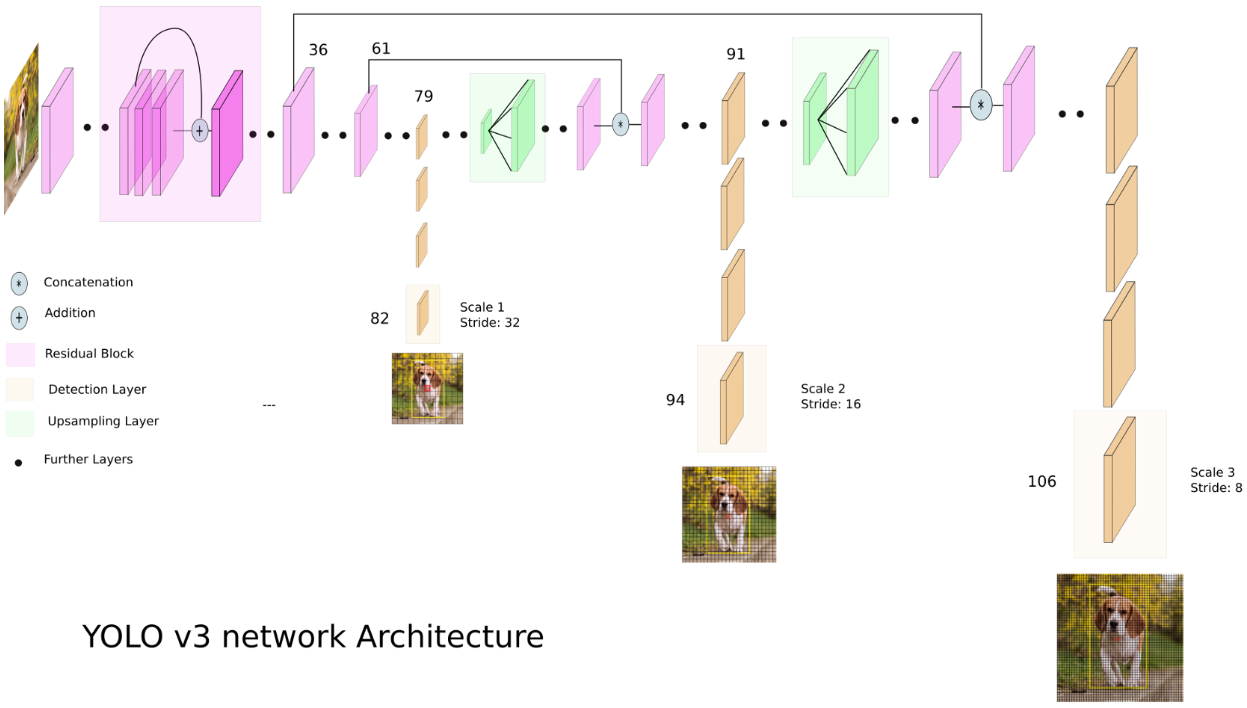
\includegraphics[width=0.85\textwidth]{yolonet.png}
\caption{Yolo Neural Network scheme.
}
\label{fig:yolo}
\end{figure}
\end{center}

The YOLO Neural Network architecture was firstly published in the 2015 but from the first version many improvements were performed and now we have the third revision of it.
We do not want to recall the history of this model so we will discuss only about the YOLOv3 model (for sake of simplicity we will call it just YOLO).

YOLO is a deep Neural Network model with more than 100 layers and more than 62 billion of parameters.
The first versions of YOLO are based on a Darknet-19 architecture (19-layer network followed by 11 more layers for object detection).
In the last release of YOLO model the first part of the network structure is used for the feature map extraction and it is essentially a modified version of the Darknet-53 model, i.e the update version of the previous model, with more layers and parameters.
This improvements increase the classification performances but it throwbacks a reduction in computational performances\footnote{
For the record, the older YOLO version are faster than the last release but less accurate.
}.
This improvement could be done also thanks to the introduction of multiple residual blocks which, as discussed in the previous sections (ref. \ref{NN:shortcut}) allows to increase the deep of the model without losing performances.

YOLO performs the object detection using a multi-scale approach: three different scales were taken into account during the training section and it increases the classification performances of the model.
The network structure can be broadly summarize as a simple CNN and its output is generated by applying a series of three different detection kernel $1\times1$ kernel on the feature map.
Moreover, this detection was performed in three different places in the network, i.e three YOLO detection layers are distributed along the network structure.
The shape of the detection kernel is $1\times1\times(B\times(5 + C))$, where $B$ is the number of bounding boxes a cell on the feature map can predict and $C$ is the number of classes.
The fixed number (\quotes{5}) is given by 4 bounding box attributes plus one object confidence coefficient (the so-called \emph{objectness} into the code).
In our applications we used the COCO dataset (see next sections, \ref{obj_detection:coco}) and thus we fixed the values of $B$ and $C$ to 3 and 80, respectively (thus the kernel size is equal to $1\times1\times255$).
We would stress that the three scale detections are equivalent to three level of down-sampling of the original image (or better the feature map), respectively equal to 32, 16 and 8.

The input image is down sampled using the first 81 layer and only the 82nd layer performs the first detection\footnote{
  Considering an input image of size $416\times416$ the resulting feature map would be of size $13\times13$.
}.
Then the feature map produced by the 79th layer is subjected to a few convolutional layers before being up sampled by 2x to a $26\times26$.
The up-sampling is performed by a previously discussed Upsample function (ref. \ref{SR:downsampling}).
The feature map is then concatenated with the one produced by the 61st layer and processed by a second series of convolutions until the 94th layer performs the second detection.
A third (similar) procedure is performed again until the end of the architecture (106th layer) where the final $52\times52\times255$ feature map is produced as output.
The first detection layer is responsible for detecting larger objects while the second two analyzes smaller regions: a comparative analysis of these three different scale results improves the detection performances and help to filter false positive cases.

The introduction of three different detection layers improves the issues of detection small objects in comparison to the previous versions but it remains a crucial limit of the model.
Moreover, the up-sampling layers connected with the previous layers (shortcut) help to preserve the fine grained features and thus the identification of small objects into the image.

The model uses a total of 9 anchor boxes with three scale per each.
The anchors have to be computed before the training phase on the training dataset: the author suggests to use a K-Means clustering for this purpose.
The first three anchors will be associated to the first (larger scale) detection layer and so on along all the structure.
Taking into account an image of $416\times416$ as example, the number of predicted boxes will be 10'647 (which is 10x the number of boxes predicted by the previous version of the model).

A further innovative improvement was given by the loss function used to train the model.
The loss computation for true positive identification has to take into account that multiple bounding boxes per grid cell are performed and thus we have to filter them.
In other words we want to preserve only the bounding boxes \quotes{responsible} for the object.
This can be achieved using the highest IoU (\emph{Intersection Over Union}) with the ground truth.
YOLO uses a modified MSE error between the predictions and the ground truth.
In particular the loss function is composed by three terms: the classification loss, the localization loss and the confidence loss.

The classification loss quantify the error of detection and it is given by

$$
\mathcal{L}_1 = \sum_{i=0}^{S^2} {\mathds{1}_i}^{\mbox{obj}} \sum_{c \in \mbox{classes}} \left(p_i(c) - \hat{p_i}(c)\right)^2
$$
\\where ${\mathds{1}_i}^{\mbox{obj}}$ is equal to 1 if an object appears in cell $i$, $p_i(c)$ is the output of the model and $\hat{p_i}(c)$ denotes the conditional class probability for class $c$ in cell $i$.

The localization loss measures the errors in the predicted boundary box locations and sizes: in this way we can filter only the boxes responsible for detecting the object.

$$
\mathcal{L}_2 = \lambda_{\mbox{coord}} \sum_{i=0}^{S^2}\sum_{j=0}^B {\mathds{1}_i}^{\mbox{obj}} \left[ (x_i - \hat{x_i})^2 + (y_i - \hat{y_i})^2 \right] +
$$
$$
\lambda_{\mbox{coord}} \sum_{i=0}^{S^2}\sum_{j=0}^B {\mathds{1}_i}^{\mbox{obj}} \left[ (\sqrt{w_i} - \sqrt{\hat{w_i}})^2 + (\sqrt{h_i} - \sqrt{\hat{h_i}})^2 \right]
$$
\\
where ${\mathds{1}_i}^{\mbox{obj}}$ is equal to 1 if $j$th boundary box in cell $i$ is responsible for detecting the object, $\lambda_{\mbox{coord}}$ increase the weight for the loss in the boundary box coordinates\footnote{
  The default value used in the model is 5.
} and $(x, y, w, h)$ are the boundary box coordinates.

The confidence loss quantifies if an object is detected into the founded box (\emph{objecteness}), i.e

$$
\mathcal{L}_2 = \sum_{i=0}^{S^2}\sum_{j=0}^B {\mathds{1}_i}^{\mbox{obj}} \left(C_i - \hat{C_i} \right)^2
$$
\\
where $\hat{C_i}$ is the box confidence score of the box $j$ in cell $i$.
If the object is not detected into the box, the confidence loss is computed as:

$$
\mathcal{L}_2 = \lambda_{\mbox{noobj}}\sum_{i=0}^{S^2}\sum_{j=0}^B {\mathds{1}_i}^{\mbox{obj}} \left(C_i - \hat{C_i} \right)^2
$$
\\
where $\lambda_{\mbox{noobj}}$ weights down the loss when detecting background (most boxes do not contain any objects and in the training images a large amount of pixels are occupied by background)\footnote{
  The default value used in the model is 0.5.
}.

The final loss is given by the sum of these three contributions

$$
\mathcal{L} = \mathcal{L}_1 + \mathcal{L}_2 + \mathcal{L}_3
$$

To further improve the detection performances we have to remove duplicate detections.
This is performed by YOLO model applying a non-maximal suppression to remove duplicates with lower confidence.
Thus, the method sorts the predictions according to the confidence scores and starting from the top scorer it filters the predictions with the same class and a IoU score greater than a given threshold.
In this way we tune the bounding boxes to be as much fit as possible to the object shape.

\end{document}
